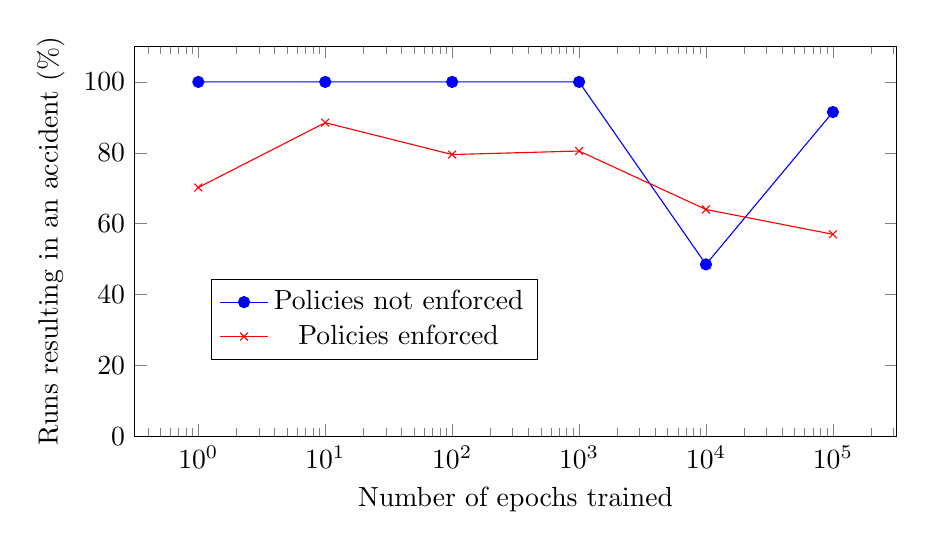
\begin{tikzpicture}
\begin{semilogxaxis}[
xlabel={Number of epochs trained},
ylabel={Runs resulting in an accident (\%)},
x=0.7cm,
y=0.45mm, 
ymin=0,
legend style={at={(0.1,0.3)},anchor=west}]

\addplot[color=blue,mark=*] coordinates {
	(0, 100)
	(1, 100)
	(10, 100)
	(100, 100)
	(1000, 100)
	(10000, 48.5)
	(100000, 91.5)
};

\addplot[color=red,mark=x] coordinates {
	(0, 75.7)
	(1, 70.2)
	(10, 88.5)
	(100, 79.5)
	(1000, 80.5)
	(10000, 64)  
	(100000, 57) 
};

\legend{Policies not enforced, Policies enforced}
\end{semilogxaxis}%
\end{tikzpicture}%